\subsection*{Problema 27}
\textbf{Enunciado:} Calcular la integral:
\begin{align*}
    I = \int \dfrac{dx}{1 + \cos^2 x}
\end{align*}

\textbf{Solución:} Siguiendo las indicaciones, dividimos el numerador y el denominador entre $\cos^2 x$:
\begin{align*}
    I &= \int \dfrac{\dfrac{1}{\cos^2 x} dx}{\dfrac{1}{\cos^2 x} + \dfrac{\cos^2 x}{\cos^2 x}} \\
    I &= \int \dfrac{\sec^2 x \, dx}{\sec^2 x + 1}
\end{align*}

Utilizamos la identidad trigonométrica fundamental $\sec^2 x = 1 + \tan^2 x$ en el denominador:
\begin{align*}
    I &= \int \dfrac{\sec^2 x \, dx}{(1 + \tan^2 x) + 1} \\
    I &= \int \dfrac{\sec^2 x \, dx}{\tan^2 x + 2}
\end{align*}

Aplicamos el cambio de variable sugerido $u = \tan x$, cuya derivada es $du = \sec^2 x \, dx$:
\begin{align*}
    I &= \int \dfrac{du}{u^2 + (\sqrt{2})^2}
\end{align*}

Esta es una integral estándar que da como resultado una función arcotangente:
\begin{align*}
    I &= \dfrac{1}{\sqrt{2}} \arctan\left(\dfrac{u}{\sqrt{2}}\right) + C
\end{align*}

Reemplazamos $u = \tan x$ para volver a la variable original:
\begin{align*}
    I = \dfrac{1}{\sqrt{2}} \arctan\left(\dfrac{\tan x}{\sqrt{2}}\right) + C
\end{align*}

\begin{figure}[H]
	\centering
	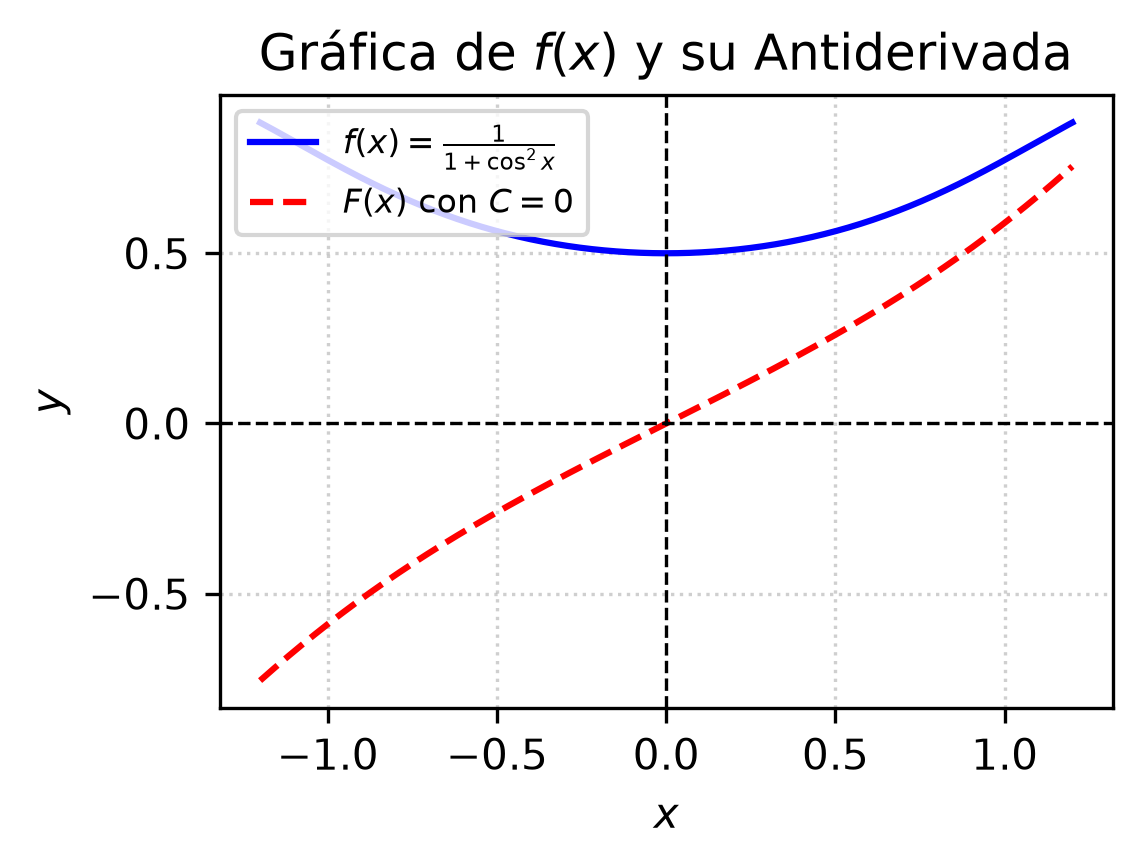
\includegraphics[width=\columnwidth]{semana_04/graficas/SEM04_P27_grafica.png}
	\caption{Representación gráfica de $f(x)$ y su antiderivada $F(x)$ evaluada para la constante de integración $C = 0$ (Problema 27).}
	\label{fig:problema27}
\end{figure}
